\documentclass{article}

\title{Machine Learning Engineer Nanodegree}
\author{Daniel Valcarce}
\usepackage{hyperref}
\usepackage{xcolor}
\usepackage{array}
\usepackage{graphicx}
\usepackage{subcaption}
\hypersetup{colorlinks,linkcolor={red!50!black}, citecolor={blue!50!black}, urlcolor={blue!80!black}}

\renewcommand{\thesection}{\Roman{section}} 
\renewcommand{\thesubsection}

\graphicspath{{images/}}

\begin{document}
	\pagenumbering{gobble}
	\maketitle
	\newpage
	\pagenumbering{arabic}
	
	\section{Definition}
	\subsection{Project Overview}
	According to the World malaria report \footnote{\label{malaria_report}\url{https://www.who.int/malaria/media/world-malaria-report-2018/en/}} , in 2017, an estimated 219 million cases of malaria
	occurred worldwide (95\% confidence interval [CI]: 203–262 million), compared with 239
	million cases in 2010 (95\% CI: 219–285 million) and 217 million cases in 2016 (95\% CI: 200–259
	million).
	
	\medskip
	In 2017, there were an estimated 435 000 deaths from malaria globally, compared with
	451000 estimated deaths in 2016, and 607000 in 2010. Nearly 80\% of global malaria deaths in
	2017 were concentrated in 17 countries in the WHO African Region and India; 7 of these
	countries accounted for 53\% of all global malaria deaths.

	\subsection{Problem Statement}
	In order to reduce the burden for microscopists in resource-constrained regions and improve
	diagnostic accuracy, the \textit{National Library of Medicine}\footnote{\label{nlm_web}\url{https://www.nlm.nih.gov/}} provide us with a dataset\footnote{\label{dataset}\url{https://ceb.nlm.nih.gov/proj/malaria/cell_images.zip}} with which I
	will create a model to detect malaria parasite in thin blood smear images.
	
	\medskip
	A common approach to create similar models consist in resize the images to a common size in order to train the model, then use this model to predict and classify new images. In this project I will apply a technique called \textbf{Progressive resizing} which consist of training different models for different size of images.
	
	\medskip
	The idea behind this technique is to create different models for different image sizes. First I need to decide which sizes could be good to train the model based on the data exploration, then I'll create and train a model with the images resized to the lower size I chose. Once the first model is trained, I will apply transfer learning to create and train the second model with the next size for the images, and so on with all Once the first model is trained, I will apply transfer learning to create and train the second model with the next size for the images, and so on with all chosen sizes.
	
	\medskip
	For each model I will get different metrics in order to know which model performs better and also to know if this technique is useful for this dataset.
	
	\subsection{Metrics}
	This project is based on the research article \textit{"Pre-trained convolutional neural networks as feature extractors toward improved malaria parasite detection in thin blood smear images"}\footnote{\label{research_paper}\url{https://www.ncbi.nlm.nih.gov/pmc/articles/PMC5907772/}} where r Rajaraman S and his
	team shown a table\footnote{\label{table_metrics}\url{https://www.ncbi.nlm.nih.gov/pmc/articles/PMC5907772/table/table-6/}} with the performance metrics results obtained during their experiments,
	comparing their custom model against other well-known models like AlexNet, VGG-16,
	ResNet-50, Xception and DenseNet-121.
	
	\medskip
	For this project I will use the same metrics and then compare the results against the values of
	their custom model.		
	
	\begin{table}[h!]
		\begin{center}
			\caption{Metrics}
			{\renewcommand{\arraystretch}{2}%
			\begin{tabular}{l|c}
				\textbf{Name} & \textbf{Formula} \\
				\hline
				Accuracy & $ \frac{TP + TN}{TP + TN + FP + FN} $ \\
				AUC & formula \\
				Sensitivity & $ \frac{TP}{TP + FN} $ \\
				Specificity & $ \frac{TN}{TN + FP} $ \\
				F1-score & $ \frac{2TP}{2TP + FP + FN} $ \\
				MCC & $ \frac{TP \times TN - FP \times FN}{\sqrt{(TP + FP)(TP + FN)(TN + FP)(TN + FN)}} $ \\
			\end{tabular}} \quad
		\end{center}
	\end{table}

\newpage

	\section{Analysis}
	\subsection{Data Exploration}	
	The dataset contains a total of 27560 images separated in two folders, Parasitized folder and
	Uninfected folder with 13780 images each.
	
	\medskip
	The image sizes varies between 49x58 and 349x241 pixels.
	
	\begin{figure}[h!]
		\centering
		\begin{subfigure}[b]{0.4\linewidth}
			\centering
			\captionsetup{justification=centering}
			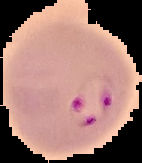
\includegraphics[width=3cm, height=3cm]{parasitized.png}
			\caption{Parasitized cell}
		\end{subfigure}\quad
		\begin{subfigure}[b]{0.4\linewidth}
			\centering
			\captionsetup{justification=centering}
			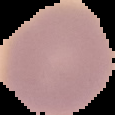
\includegraphics[width=3cm, height=3cm]{uninfected.png}
			\caption{Uninfected cell}
		\end{subfigure}
		\caption{Dataset sample}
		\label{fig:cells}
	\end{figure}

	\subsection{Exploratory Visualization}
	
	
\end{document}